\documentclass[a4paper,11pt]{article}
\usepackage[utf8]{inputenc}
\usepackage{xcolor}
\usepackage{amsmath}
\usepackage{amssymb}
\usepackage{tikz}
\usetikzlibrary{patterns}

\begin{document}

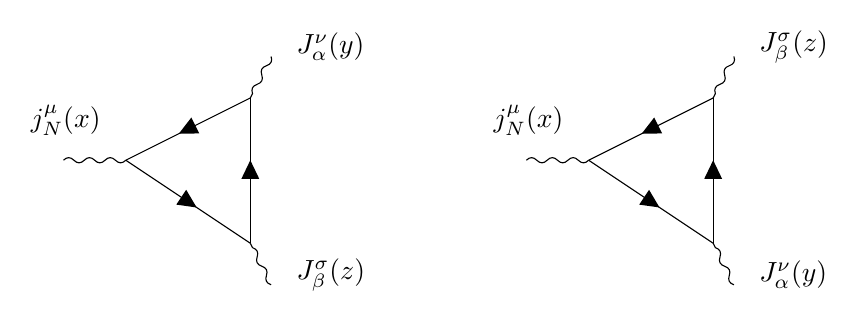
\begin{tikzpicture}[x=0.75pt,y=0.75pt,yscale=-1,xscale=1]

\draw    (188,70) -- (248,110) ;
\draw [shift={(222.16,92.77)}, rotate = 213.69] [fill={rgb, 255:red, 0; green, 0; blue, 0 }  ][line width=0.08]  [draw opacity=0] (8.93,-4.29) -- (0,0) -- (8.93,4.29) -- cycle    ;
\draw    (248,40) -- (188,70) ;
\draw [shift={(213.53,57.24)}, rotate = 333.43] [fill={rgb, 255:red, 0; green, 0; blue, 0 }  ][line width=0.08]  [draw opacity=0] (8.93,-4.29) -- (0,0) -- (8.93,4.29) -- cycle    ;
\draw    (248,110) -- (248,40) ;
\draw [shift={(248,70)}, rotate = 90] [fill={rgb, 255:red, 0; green, 0; blue, 0 }  ][line width=0.08]  [draw opacity=0] (8.93,-4.29) -- (0,0) -- (8.93,4.29) -- cycle    ;
\draw    (188,70) .. controls (186.33,71.67) and (184.67,71.67) .. (183,70) .. controls (181.33,68.33) and (179.67,68.33) .. (178,70) .. controls (176.33,71.67) and (174.67,71.67) .. (173,70) .. controls (171.33,68.33) and (169.67,68.33) .. (168,70) .. controls (166.33,71.67) and (164.67,71.67) .. (163,70) .. controls (161.33,68.33) and (159.67,68.33) .. (158,70) -- (158,70) ;
\draw    (258,20) .. controls (258.75,22.24) and (258,23.73) .. (255.76,24.47) .. controls (253.53,25.22) and (252.78,26.71) .. (253.53,28.94) .. controls (254.28,31.18) and (253.53,32.67) .. (251.29,33.42) .. controls (249.06,34.17) and (248.31,35.66) .. (249.06,37.89) -- (248,40) -- (248,40) ;
\draw    (258,130) .. controls (255.76,129.26) and (255.01,127.77) .. (255.76,125.53) .. controls (256.51,123.3) and (255.76,121.81) .. (253.53,121.06) .. controls (251.29,120.31) and (250.54,118.82) .. (251.29,116.58) .. controls (252.04,114.35) and (251.29,112.86) .. (249.06,112.11) -- (248,110) -- (248,110) ;
\draw    (411,70) -- (471,110) ;
\draw [shift={(445.16,92.77)}, rotate = 213.69] [fill={rgb, 255:red, 0; green, 0; blue, 0 }  ][line width=0.08]  [draw opacity=0] (8.93,-4.29) -- (0,0) -- (8.93,4.29) -- cycle    ;
\draw    (471,40) -- (411,70) ;
\draw [shift={(436.53,57.24)}, rotate = 333.43] [fill={rgb, 255:red, 0; green, 0; blue, 0 }  ][line width=0.08]  [draw opacity=0] (8.93,-4.29) -- (0,0) -- (8.93,4.29) -- cycle    ;
\draw    (471,110) -- (471,40) ;
\draw [shift={(471,70)}, rotate = 90] [fill={rgb, 255:red, 0; green, 0; blue, 0 }  ][line width=0.08]  [draw opacity=0] (8.93,-4.29) -- (0,0) -- (8.93,4.29) -- cycle    ;
\draw    (411,70) .. controls (409.33,71.67) and (407.67,71.67) .. (406,70) .. controls (404.33,68.33) and (402.67,68.33) .. (401,70) .. controls (399.33,71.67) and (397.67,71.67) .. (396,70) .. controls (394.33,68.33) and (392.67,68.33) .. (391,70) .. controls (389.33,71.67) and (387.67,71.67) .. (386,70) .. controls (384.33,68.33) and (382.67,68.33) .. (381,70) -- (381,70) ;
\draw    (481,20) .. controls (481.75,22.24) and (481,23.73) .. (478.76,24.47) .. controls (476.53,25.22) and (475.78,26.71) .. (476.53,28.94) .. controls (477.28,31.18) and (476.53,32.67) .. (474.29,33.42) .. controls (472.06,34.17) and (471.31,35.66) .. (472.06,37.89) -- (471,40) -- (471,40) ;
\draw    (481,130) .. controls (478.76,129.26) and (478.01,127.77) .. (478.76,125.53) .. controls (479.51,123.3) and (478.76,121.81) .. (476.53,121.06) .. controls (474.29,120.31) and (473.54,118.82) .. (474.29,116.58) .. controls (475.04,114.35) and (474.29,112.86) .. (472.06,112.11) -- (471,110) -- (471,110) ;

% Text Node
\draw (141,42.4) node [anchor=north west][inner sep=0.75pt]    {$j_{N }^{\mu }(x)$};
% Text Node
\draw (269,7.4) node [anchor=north west][inner sep=0.75pt]    {$J_{\alpha }^{\nu }( y)$};
% Text Node
\draw (269,116.4) node [anchor=north west][inner sep=0.75pt]    {$J_{\beta }^{\sigma }(z)$};
% Text Node
\draw (364,42.4) node [anchor=north west][inner sep=0.75pt]    {$j_{N }^{\mu }(x)$};
% Text Node
\draw (492,117.4) node [anchor=north west][inner sep=0.75pt]    {$J_{\alpha }^{\nu }( y)$};
% Text Node
\draw (492,6.4) node [anchor=north west][inner sep=0.75pt]    {$J_{\beta }^{\sigma }(z)$};


\end{tikzpicture}

\end{document}